

\documentclass[8pt, usepdftitle=false]{beamer}
% \imput{../common/beamerthemesimple}
\usetheme{simple}


  \usepackage{xcolor}
  \definecolor{olive}{rgb}{0.3, 0.4, .1}
  \setbeamercolor{itemize/enumerate body}{fg=black}
  \setbeamercolor{title}{fg = green!30!black}
  \setbeamercolor{frametitle}{fg = gray!70!black, bg = white}


% \usepackage{lmodern}
\usepackage[scale = 2]{ccicons}
\usepackage[export]{adjustbox}
\usepackage{amsmath, amsthm, amssymb}
\usepackage{amsfonts}
\usepackage{mathtools}

\usepackage[justification=raggedright,width=\linewidth]{caption}
\usepackage{tikz} 


\usepackage{setspace}

\setbeamertemplate{title page}[default][right,colsep=-4bp,rounded=true,shadow=\beamer@themerounded@shadow]

\setbeamertemplate{caption}[numbered]


%% Options

\setbeamercolor{alerted text}{fg=blue}
\setbeamertemplate{alerted text begin}{\itshape}
\setbeamertemplate{alerted text end}{}

\newenvironment<>{varblock}[2][\textwidth]{%
    \setlength{\textwidth}{#1}
    \begin{actionenv}#3%
        \def\insertblocktitle{\underline{#2}}%
        \par%
        \usebeamertemplate{block begin}}
        {\par%
        \usebeamertemplate{block end}%
    \end{actionenv}}

\setbeamertemplate{blocks}[rounded][shadow=true]
\setbeamercolor{block title}{fg=black,bg=gray!20!white}
\setbeamercolor{block body}{fg=black,bg=gray!10!white}




%% Theorem

% \newtheorem{theorem}{Theorem}

%% Bangla tex


\usepackage{polyglossia}
\setotherlanguage[numerals=Devanagari]{bengali}
\setmainlanguage{english}
\newfontfamily\bengalifont[Script=Bengali]{Akaash}


%% tikx

\usepackage{tikz}
\usetikzlibrary{calc,trees,positioning,arrows,fit,shapes,calc}





\newcommand\blfootnote[1]{%
  \begingroup
  \renewcommand\thefootnote{}\footnote{#1}%
  \addtocounter{footnote}{-1}%
  \endgroup
}



\newcommand\Permute[2][^n]{\prescript{#1\mkern-2.5mu}{}P_{#2}}
\newcommand\Combine[2][^n]{\prescript{#1\mkern-0.5mu}{}C_{#2}}


\renewcommand*{\thefootnote}{\fnsymbol{footnote}}


\usepackage{flexisym}
\usepackage{breqn}

\usepackage[T1]{fontenc}

% \usepackage{mathpazo}
% \renewcommand{\rmdefault}{put}

% \usepackage{fourier} 
% Only use the math font of mathpazo
% \let\temp\rmdefault
% \usepackage{mathpazo}
% \let\rmdefault\temp
% \renewcommand{\rmdefault}{put}


% \usepackage[hyphens]{url}


  % \usefonttheme{professionalfonts} % using non standard fonts for beamer
  % \usefonttheme{serif} % default family is serif

  % \usepackage{gentium}
  \usepackage{multicol}
  \usepackage{mathpazo}



% \renewcommand{\familydefault}{\sfdefault}  


  % color brackets
  \makeatletter
  \newcount\bracketnum
  \newcommand\makecolorlist[1]{%
      \bracketnum0\relax
      \makecolorlist@#1,.%
      \bracketnum0\relax
  }
  \def\makecolorlist@#1,{%
      \advance\bracketnum1\relax
      \expandafter\def\csname bracketcolor\the\bracketnum\endcsname{\color{#1}}%
      \@ifnextchar.{\@gobble}{\makecolorlist@}%
  }
  \let\oldleft\left
  \let\oldright\right
  \def\left#1{%
      \global\advance\bracketnum1\relax 
      \colorlet{temp}{.}%
      \csname bracketcolor\the\bracketnum\endcsname
      \oldleft#1%
      \color{temp}%
  }
  \def\right#1{%
      \colorlet{temp}{.}%
      \csname bracketcolor\the\bracketnum\endcsname
      \oldright#1%
      \global\advance\bracketnum-1\relax
      \color{temp}%
  }
  \makeatother


  \makecolorlist{black,blue,red}






\setbeamertemplate{section in toc}{%
  {\color{firstcolor}\inserttocsectionnumber.}~\inserttocsection}
\setbeamercolor{subsection in toc}{bg=white,fg=black}
\setbeamertemplate{subsection in toc}{%
  \hspace{1.2em}{\color{firstcolor}\rule[0.3ex]{3pt}{3pt}}~\inserttocsubsection\par}


\setbeamerfont{section in toc}{size=\fontsize{6}{8}\selectfont}
\setbeamerfont{subsection in toc}{size=\fontsize{6}{8}\selectfont}
\setbeamerfont{subsection in toc shaded}{size=\fontsize{6}{8}\selectfont}


\makeatletter
\patchcmd{\beamer@sectionintoc}{\vskip1.5em}{\vskip0.5em}{}{}
\makeatother






  \usepackage{twemojis}
  \usepackage{fontspec}
  \usepackage{tikzsymbols}
  \newfontfamily\DejaSans{DejaVu Sans}

% for R
\usepackage[fixed]{fontawesome5}


\setbeamercolor{emph}{fg=red}
\renewcommand<>{\emph}[1]{%
  {\color{purple}\only#2{\rm\itshape}#1}%
}

\setbeamertemplate{frametitle continuation}{}


\usepackage[round,  maxcitenames=10, mincitenames=11]{natbib}
\setlength{\bibhang}{0pt}
\renewcommand{\bibsection}{}
\usepackage{fancybox}


\setbeamertemplate{section page}
{
    \begingroup
    \begin{beamercolorbox}[sep=12pt,center]{section title}
        \usebeamerfont{section title}\insertsection\par
    \end{beamercolorbox}
    \endgroup
}

\setbeamertemplate{subsection page}
{
    \begingroup
    \begin{beamercolorbox}[sep=12pt,center]{section title}
        \usebeamerfont{section title}\insertsection\par
    \end{beamercolorbox}
    \vspace*{-1pt}
    \begin{beamercolorbox}[sep=8pt,center]{subsection title}
        \usebeamerfont{subsection title}\insertsubsection\par
    \end{beamercolorbox}
    \endgroup
}



\newcommand\Var[1]{\mathbb{V}\mathrm{ar}{#1}}



\renewcommand{\emph}[1]{%
{\rm\itshape{\color{purple}#1}}%
}

\renewcommand{\alert}[1]{%
{\rm\itshape{\color{blue}#1}}%
}

\newcounter{mytheorem}
\renewcommand{\themytheorem}{4.\arabic{mytheorem}}
\newcommand{\Thm}[1]{\refstepcounter{mytheorem}\textbf{#1\color{blue}\themytheorem}:}




%================ Give the title ============================##

\title{\LARGE Ch4 - Probability Theory - 3 }

\subtitle{{\fontsize{10}{10}\selectfont\color{gray!50!balck}
(Short Chapter on Joint Distributions)} 
\\\vspace*{.2cm}Statistics For Business and Economics - I}

\author{Shaikh Tanvir Hossain\vspace*{-.4cm}}

\institute{ East West University, Dhaka\\ Last Updated \today}
\date{\vspace{-5pt}}
% \titlegraphic{
\includegraphics[width=300,height=.5\textheight]{Images/EWU.png}}

% \setbeamertemplate{background}{\tikz[overlay,remember picture]\node[opacity=0.90]at (current page){
\includegraphics[width=.5\textwidth,left]{EWU.png}};}

\usepackage{hyperref}
\hypersetup{
      pdftitle={Ch4 - Probability Theory - 3},
        pdfauthor={Shaikh Tanvir Hossain},
          pdfborder={0 0 0},
       colorlinks,
      citecolor=blue,
      linkcolor=gray!50!black,
    breaklinks=true}






\begin{document}

% input the outline 

\begin{frame}[plain,noframenumbering] 
    \maketitle
\end{frame}
\setbeamertemplate{background}{}
\setlength{\abovedisplayskip}{-2pt}
\setlength{\belowdisplayskip}{4pt}
\setlength{\abovedisplayshortskip}{-3pt}
\setlength{\belowdisplayshortskip}{4pt}


\AtBeginSection[]
{
    \begin{frame}[plain, allowframebreaks]
\setstretch{.1}

        \setlength{\parskip}{1ex}
            \tableofcontents[sections={1-7}, 
            currentsubsection, 
            sectionstyle=show/hide, 
            sectionstyle=show/shaded, 
            ]
    \end{frame}
}


% Hide progress bar and footline on titlepage
\begin{frame}{Outline}
 \vspace*{.2cm}

\begin{center}
\begin{minipage}{10cm}
  \begin{alertblock}{Outline}
  \setstretch{.1}
   \setlength{\parskip}{1ex}
  \tableofcontents[sections={1-10}]
  %   \framebreak
  % \tableofcontents[sections={2}]
\end{alertblock}
\end{minipage}
\end{center}


\end{frame}



\begin{frame}[allowframebreaks]{}

\begin{itemize}
\item In this chapter we will see a short overview of concepts related to joint distribution. The idea of joint probability distribution is just an application of the idea of joint probability table. Then automatically you can think about marginal probabilities and conditional probabilities. Almost all ideas are conceptually same as the ideas we saw in Chapter-2, but now this will be for multiple random variables.





\item So let's start...\faWalking \faWalking \faWalking.

\end{itemize}

\end{frame}



\section{Introduction and Examples}
\frame{\sectionpage}


\begin{frame}[allowframebreaks]{Multiple Random Variables and Joint distributions}

\begin{itemize}
  \item So far we talked about a single random variable (whether it was discrete or continuous) and its distributions. So this a \alert{univariate} setup, where we try to understand only one random variable and its distribution.

  \item But in statistics we can also think about more than a single random variable, we call this a \alert{multivariate} setup. 

  \item Multivariate setup captures how different random variables interact with each other. 

  \item The most important object in this case is their \alert{joint distribution}, which has the probabilities when multiple random variables take different values together. 


  \item We will introduce multivariate analogs of the PMF, PDF and also CDF. Like the univariate case these objects will help us to think about the probabilities for multiple random variables.

  \item Three key concepts of this section are - \alert{joint distribution, marginal distributions} and \alert{conditional distributions}.

  \item If you have understood joint probability table, conditional probabilities and marginal probabilities\footnote[frame]{This is explained in Chapter-2 and also look at PS-2}, this will be very easy for you. But if you are struggling with these concepts you should go back to Chapter-2, read and understand before you continue. 


  \item Here are some real life examples,

  \begin{itemize}
    \item 1. Suppose that we choose a \alert{random family} of Bangladesh, and we would like to study following things,

    \begin{itemize}
      \item The number of people in the family (this is a random variable $X_1$).

      \item The household income of this family (this is a random variable $X_2$).

      \item The household expenditure of this family (this is a random variable $X_3$).
    \end{itemize}

   $X_1$, $X_2$ and $X_3$ are all random variables, and it is natural that they are all related to each other.

   \item 2. Two or more stock prices - Maybe we can represent a stock price of a company with $X_1$, and a stock price of another company with $X_2$, and often different stock prices move up and down together!


   \item We will see more examples in the coming section.
  \end{itemize}

  \item Next we will start talking about Joint Distributions. We will start from looking into only two random variables, $X$ and $Y$ and their distributions together. This is called \alert{Bivariate setup}. 

  \item Bivariate distributions are easy to understand and visualize, and this helps to understand situations when we have more than two random variables.
\end{itemize}




\end{frame}



% \begin{frame}{Multiple Random Variables and Joint distributions}

% When we discussed random variables and their distributions before, we noted that the individual distributions of two random variable do not tell us anything about whether they are independent or dependent. For example, two $\operatorname{Bern}(1 / 2)$ $X$ and $Y$ could be independent if they indicate Heads on two different coin flips, or dependent if they indicate Heads and Tails respectively on the same coin flip (Try!). Thus, although the PMF of $X$ is a complete blueprint for $X$ and the PMF of $Y$ is a complete blueprint for $Y$, these individual PMFs are missing important information about how the two random variables are related.

% Now we will consider joint distributions, also called multivariate distributions, which capture the previously missing information about how multiple random variables interact. We introduce multivariate analogs of the $\mathrm{PMF}$, and $\mathrm{PDF}$ in order to provide a complete specification of the relationship between multiple random variables.


% Three key concepts of this section: \emph{joint, marginal} and \emph{conditional distributions}

% \begin{itemize}
%   \item \textbf{Joint Distriution} - The joint distribution of two random variables $X$ and $Y$ provides complete information about the probability of the vector $(X, Y)$ falling into any subset of the plane. 

  
%   \item \textbf{Marginal Distriution}- The marginal distribution of $X$ is the individual distribution of $X$, ignoring the value of $Y$
%   \item \textbf{Conditional Distriution} - the conditional distribution of $X$ given $Y=y$ is the updated distribution for $X$ after observing $Y=y$. 


% \end{itemize}

% We'll formally look at these concepts in the discrete case first, then extend them to the continuous case.

% \end{frame}


\section{Joint, Marginal and Conditional Distributions}


\subsection{Joint PMF or PDF}




\begin{frame}{Joint Distribution}




\begin{itemize}

\item Let's start with our familiar example from Chapter-2, recall, 


\begin{table}
\centering
  \begin{tabular}{|lccccc|}
\hline & \multicolumn{4}{c}{ Treatment group } & \\
\cline { 2 - 6 } Response & Imipramine & Lithium & Combination & Placebo & Total \\
\hline Relapse & 18 & 13 & 22 & 24 & 77 \\
No relapse & 22 & 25 & 16 & 10 & 73 \\
\hline Total & 40 & 38 & 38 & 34 & 150 \\
\hline
\end{tabular}
\end{table}


\item From here we can easily calculate the joint probability table, 


\begin{table}
\centering
  \begin{tabular}{|lcccc|c|}
\hline & \multicolumn{4}{c}{ Treatment group } & \\
\cline { 2 - 6 } Response & Imipramine & Lithium & Combination & Placebo & Total \\
\hline Relapse & 0.12 & 0.08 & 0.15 & 0.16 & 0.51 \\
No relapse & 0.15 & 0.17 & 0.10 & 0.07 & 0.49 \\
\hline Total & 0.27 & 0.25 & 0.25 & 0.23 & 1 \\
\hline
\end{tabular}
\end{table}

\item Important: We only took decimal places upto two digits, so there might be some rounding errors.



  
\end{itemize}


\end{frame}






\begin{frame}{Joint Distribution}




\begin{itemize}

\item Let's introduce two random variables, $X$ and $Y$....Random variables just take things to real numbers.

\item $X$ represents treatment group -  

\begin{itemize}

 \item $1$ for Imipramine
 \item $2$ for Lithium
 \item  $3$ for Combination
 \item $4$ for Placebo

\end{itemize}


\item $Y$ represents response condition -  
 


\begin{itemize}

 \item $1$ means patient had a relapse
 \item $0$ means patient didn't have a relapse

 
\end{itemize}

\item Now we can write following joint probability distribution


\begin{table}
\centering
  \begin{tabular}{|lcccc|c|}
\hline & \multicolumn{4}{c}{ Treatment group ($X$) } & \\
\cline { 2 - 6 } Response ($Y$) & 1 & 2 & 3 & 4 & Total \\
\hline 1 & 0.12 & 0.08 & 0.15 & 0.16 & 0.51 \\
0 & 0.15 & 0.17 & 0.10 & 0.07 & 0.49 \\
\hline Total & 0.27 & 0.25 & 0.25 & 0.23 & 1 \\
\hline
\end{tabular}
\end{table}

\item Note in this case both of the variables are discrete random variables.


\item Here $\mathbb{P}(X = 1, Y = 0) = 0.15$ means if we randomly select one individual from the \alert{population of $150$}, then there is a $15\%$ chance that he/she had Imipramine and she didn't have a relapse (can you give a frequency interpretation, think about if you pcik randomly an individual $100$ times from this population?)
  
\end{itemize}


\end{frame}



\begin{frame}{Joint PMF}



\begin{itemize}

 \item The last example is an example of \alert{joint probability distribution} of two discrete random variables $X$ and $Y$.

 \item Note that in this case we have all $6$ probabilities,

 \begin{itemize}
   \item $\mathbb{P}(X = x, Y = y)$, where possible values of $x$ are $1, 2, 3$ and possible values of $y$ are $0, 1$.

   \item You can check that these probabilities will sum to $1$.

   \item This means $  \sum_x \sum_y \mathbb{P}(X = x, Y = y)=1$
 \end{itemize}

 \item What does double sum mean? Ans: This means we are summing over all $x$ and $y$ values.

 \item Now since these are discrete probabilities, we can also think about an underlying joint PMF or \alert{joint probability mass function}.

 \item The idea of the joiny PMF is same as univariate PMF, it's just a PMF for all combinations of values.



\end{itemize}


\end{frame}


\begin{frame}{Joint PMF}


\begin{varblock}{\Thm{Definition } (Joint PMF of two random variables)}

The joint PMF of discrete random variables $X$ and $Y$ is the function $f(x, y)$ given by

\begin{align*}
f(x, y)=\mathbb{P}(X=x, Y=y) .
\end{align*}

\end{varblock}

\begin{itemize}
  \item As you can alreasy guess, for a valid joint PMFs, the values must be nonnegative and they should be summed to 1, so
  \begin{align*}
  \sum_x \sum_y f(x,y)=1
  \end{align*}
  \item The joint PMF determines the distribution (or it is sufficient to know the Joint PMF if we want to know the joint distribution). This is because we can use it to find the probability of the event $(X, Y) \in A$ for any set $A$ in the $x-y$ plane or $2D$ plane. All we have to do is sum the joint PMF over $A$ :
  \begin{align*}
  \mathbb{P}((X, Y) \in A)=\underset{{(x, y) \in A}}{\sum\sum} \mathbb{P}(X=x, Y=y)
  \end{align*}
  
\end{itemize}


\end{frame}

\begin{frame}{Joint PMF}

\Thm{Example~ }

The following table gives the joint PMF of the discrete variables $X$ and $Y$.

\begin{table}
\centering
  \begin{tabular}{|lcccc|c|}
\hline & \multicolumn{4}{c}{ Treatment group ($X$) } & \\
\cline { 2 - 6 } Response ($Y$) & 1 & 2 & 3 & 4 & Total \\
\hline 1 & 0.12 & 0.08 & 0.15 & 0.16 & 0.51 \\
0 & 0.15 & 0.17 & 0.10 & 0.07 & 0.49 \\
\hline Total & 0.27 & 0.25 & 0.25 & 0.23 & 1 \\
\hline
\end{tabular}
\end{table}



From the table, we can find probabilities of all combination of values of $(X,Y)$. To check you understood the concept, you should find
\begin{itemize}
  \item $\mathbb{P}(X=2, Y=1) = ?$
  \item $\mathbb{P}(X=2, Y=0) = ?$
  \item $\mathbb{P}(X>1, Y>0) = ?$
\end{itemize}

\end{frame}

\begin{frame}{Joint PMF}

\Thm{Example~ }


Here is another example,


\begin{table}
\centering
\begin{tabular}{llllll}
\hline & & \multicolumn{4}{c}{$X$} \\
\cline { 3 - 6 } & & ${- 2}$ & ${0}$ & ${2}$ & ${3}$ \\
\hline$Y$ & ${3}$ & $0.27$ & $0.08$ & $0.16$ & 0 \\
& ${6}$ & 0 & $0.04$ & $0.10$ & $0.35$ \\
\hline
\end{tabular}
\end{table}

Try to find

\begin{itemize}
  \item $\mathbb{P}(X=2, Y=3) = ?$
  \item $\mathbb{P}(X=3, Y=3) = ?$
  \item $\mathbb{P}(X>1, Y>3) = ?$
\end{itemize}



\end{frame}


\begin{frame}{Joint PMF}
\begin{figure}
  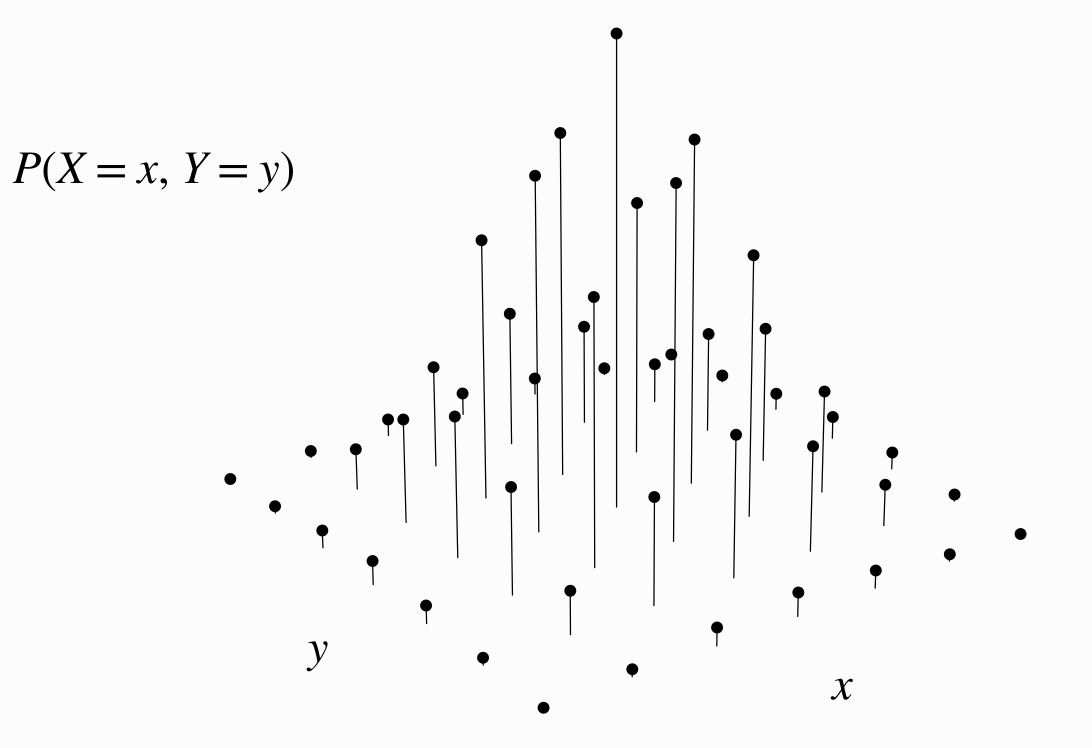
\includegraphics[scale = .25]{Images/joint_PMF.png}
  \caption{Figure above shows a sketch of what the joint PMF of two discrete random variables could look like. The height of a vertical bar at $(x, y)$ represents the probability $\mathbb{P}(X=x, Y=y)$ or $f(x, y)$. For the joint PMF to be valid, the total height of the vertical bars must be 1 .}
\end{figure}




\end{frame}


\begin{frame}[allowframebreaks]{Joint PDF}
\begin{itemize}
	\item What about Joint PDF?

	\item The idea would extend in a similar way.

	\item For example if we have two continuous random variables $X$ and $Y$, then there would be a joint density function $f(x, y)$ as follows and with that we can calculate the probabilities under the curve give a certain region

	\begin{align*}
	\mathbb{P}((X, Y) \in A)={\int \int}\limits_{(x, y) \in A} f(x, y) d x d y
	\end{align*}

	\item The double integral looks very complicated, but it is just a generalization of the sum for the discrete case. 

	\item Here we are integrating over the region $A$ in the $x-y$ plane, and the integrand is the joint PDF $f(x, y)$. 

	\item Here is an example of bi-variate normal, 

	\begin{figure}
		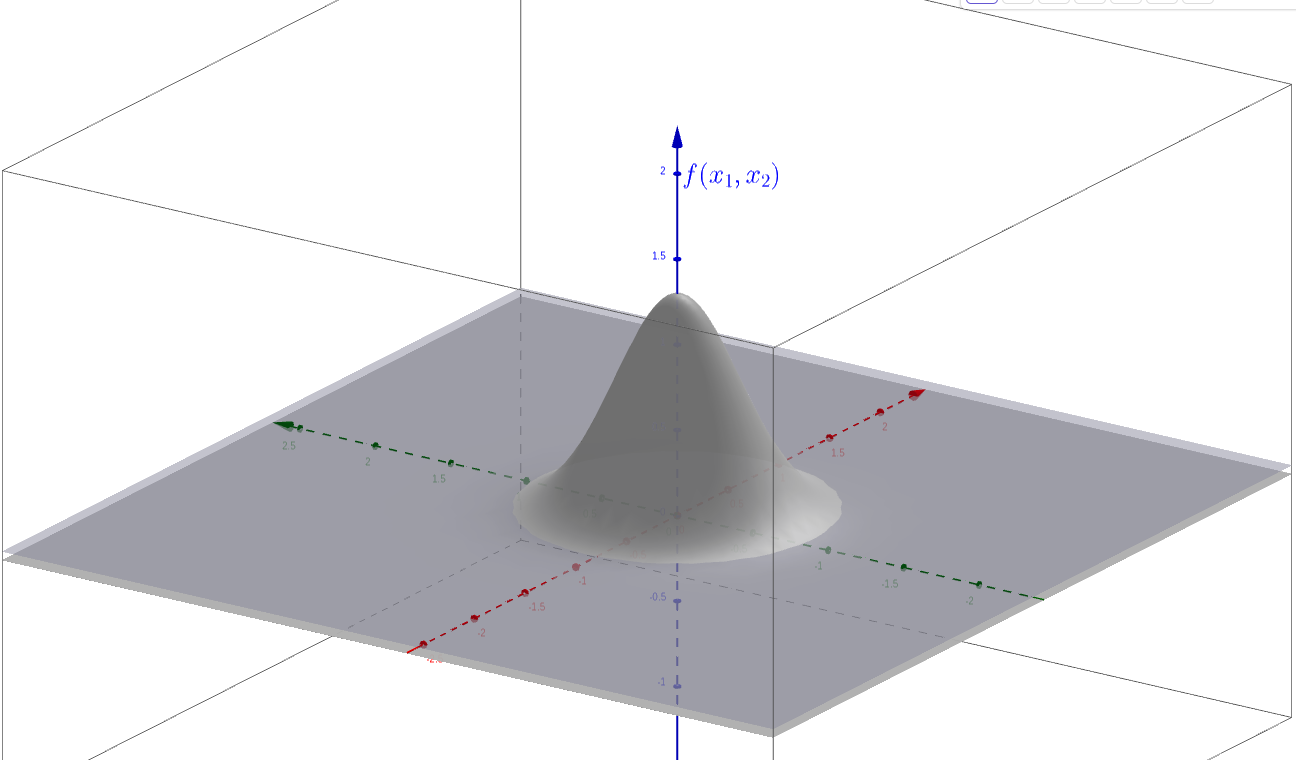
\includegraphics[scale = .2]{Images/MVnorm.png}
	\end{figure}

	\item The functions looks a bit more scary, sorry,

	\begin{align*}
		\begin{aligned}
& f_{X Y}(x, y)=\frac{1}{2 \pi \sigma_X \sigma_Y \sqrt{1-\rho^2}} \times  \\
& e^{ \left\{-\frac{1}{2\left(1-\rho^2\right)}\left[\left(\frac{x-\mu_X}{\sigma_X}\right)^2+\left(\frac{y-\mu_Y}{\sigma_Y}\right)^2-2 \rho \frac{\left(x-\mu_X\right)\left(y-\mu_Y\right)}{\sigma_X \sigma_Y}\right]\right\}}
\end{aligned}
	\end{align*}

	\item Here we have two random variables, $X$ and $Y$ which are jointly normal. Now we have $5$ parameters, $\mu_X$, $\mu_Y$, $\sigma_X$, $\sigma_Y$ and $\rho$. 

	\item We will not go into details of the joint distribution of two continuous random variables, rather we will understand using discrete random variables ... for joint the ideas extend in a similar way!







\end{itemize}


\end{frame}


\subsection{Marginal PMFs, Marginal Expectation and Marginal Variance}
\frame{\subsectionpage}


% \begin{frame}{Notations for Joint, Marginal and Conditional}

% \textbf{\color{red} Be Careful with different notations}

% \begin{itemize}

%   \item Within few slides we will have lots of PMFs, Expectations and Variance. So we need to carefully denote different objects (I am sorry previosuly the notation was a bit sloppy!)

%   \item The need for new notation is because now we have many objects.

%   \item Throughout this lecture, {\color{red}we will use following notations when we have joint probabilities of two random variables $X$ and $Y$}.

%   \item \alert{For joint PMF} we will use $f(x, y)$, so here we don't have any confusion.

%   \item \alert{For the Marginal PMF of $X$}, we will use $f_{X}(x)$ (notice the subscript $X$)

%   \item \alert{For the Marginal PMF of $Y$}, we will use $f_{Y}(y)$ (notice the subscript $Y$)

%   \item \alert{For marginal expectations and marginal variance} it's clear from the notations, so we don't need anything new, we will use usual notations $\mathbb{E}(X)$,  $\mathbb{E}(Y)$,  $\mathrm{Var}(X)$ and  $\mathrm{Var}(Y)$.
  
%   \item \alert{For the conditional PMF}, we will use $f_{\scriptscriptstyle Y|X }(y|x)$ and $f_{\scriptscriptstyle X|Y}(x|y)$. Note that depending on each conditioning value we will have a different PMF, we will see examples of this.

%   \item \alert{For conditional expectation}, we will use $\mathbb{E}(Y | X = x)$ and $\mathbb{E}(X | Y = y)$, again depending on each conditioning value we will have a different conditional expectation, we will see examples of this.

%   \item \alert{For conditional variance}, we will use we will use $\mathrm{Var}(Y | X = x)$ and $\mathrm{Var}(X | Y = y)$, and also depending on each conditioning value we will have a different conditional variance, we will see examples of this.






% \end{itemize}


% \end{frame}


\begin{frame}{Notations for Joint, Marginal and Conditional}

\textbf{\color{red} Be Careful with different notations}


\begin{itemize}

  \item Within few slides we will have lots of PMFs, Expectations and Variance. So we need to carefully denote different objects (I am sorry previosuly the notation was a bit sloppy!)

  \item The need for new notation is because now we have many objects.

  \item Throughout this lecture, {\color{red}we will use following notations when we have joint probabilities of two random variables $X$ and $Y$}.



% Please add the following required packages to your document preamble:
% \usepackage{graphicx}
\begin{table}[]
\resizebox{\textwidth}{!}{%
\begin{tabular}{l|l}
\alert{Notations}                                 & \alert{What does it mean}                                                      \\ \hline
$f(x, y)$                                         & Joint PMF                                                                      \\ \hline
$f_{X}(x)$, $\mathbb{E}(X)$ and $\mathrm{Var}(X)$ & Marginal PMF of $X$, Marginal Expectation of $X$, and Marginal Variance of $X$ \\
$f_{Y}(y)$, $\mathbb{E}(Y)$ and $\mathrm{Var}(Y)$ & Marginal PMF of $Y$, Marginal Expectation of $Y$, and Marginal Variance of $Y$ \\ \hline
$f_{\scriptscriptstyle Y|X }(y|x)$                & Conditional PMF of Y, conditioning on a fixed value $X = x$                    \\
$\mathbb{E}(Y | X = x)$                           & Conditional Expectation of Y, conditioning on a fixed value $X = x$            \\
$\mathrm{Var}(Y | X = x)$                         & Conditional Variance of Y, conditioning on a fixed value $X = x$               \\
$f_{\scriptscriptstyle X|Y}(x|y)$                 & Conditional PMF of X, conditioning on a fixed value $Y = y$                    \\
$\mathbb{E}(X | Y = y)$                           & Conditional Expectation of X, conditioning on a fixed value $Y = y$            \\
$\mathrm{Var}(X | Y = y)$                         & Conditional Variance of X, conditioning on a fixed value $Y = y$              \\ \hline
\end{tabular}%
}
\end{table}


\item Note that depending on each conditioning value we will have a different PMF, different expectation and different variance, we will see examples of this.

\end{itemize}

\end{frame}






\begin{frame}{Marginal PMF}

\begin{itemize}
  \item Now let's start talking about marginal objects first.

  \item Question is - if we have a joint PMF $f(x, y)$ (for example look at Example 3.3), can we get PMF $f_{X}(x)$ and PMF $f_{Y}(y)$? which are simply the univariate PMF of $X$ and $Y$? The answer is YES!

  \item These are called \alert{Marginal PMFs}. 

  \item For the discrete random variables $X$, we can obtain $f_{X}(x)$ by summing the joint PMF $f(x, y)$ over the possible values of $Y$ (similarly we can do it for $Y$)

  \item Here is the formal definition, don't worry we will look at some examples now.

\begin{varblock}{\Thm{Definition } (Marginal PMF)}

For discrete random variables $X$ and $Y$

\begin{itemize}
  \item The marginal PMF of $X$ is $f_{X}(x) =  \sum_y f(x,y)$.

  \item The marginal PMF of $Y$ is $f_{X}(y) =\sum_x f(x,y)$.
\end{itemize}



\end{varblock}

  \item It is important to note that the marginal PMF of $X$ is the PMF of $X$, viewing $X$ individually rather than jointly with $Y$ (similarly think about marginal PMF of $Y$) . 
 
  \item The operation of summing over the possible values of $Y$ in order to convert the joint PMF into the marginal PMF of $X$ is known as \alert{marginalization of $Y$} or \alert{marginalizing out $Y$}.



\end{itemize}


\end{frame}









\begin{frame}{Marginal PMF}
\Thm{Example~ }

Consider the table in Example 3.3. The marginal PDF of $X$, denoted by $f_{X}(x)$ is obtained as follows:

\begin{align*}
\begin{aligned}
&f_{X}(-2)=\sum_y f(x, y)=0.27+0=0.27 \\
&f_{X}(0)=\sum_y f(x, y)=0.08+0.04=0.12 \\
&f_{X}(2)=\sum_y f(x, y)=0.16+0.10=0.26 \\
&f_{X}(3)=\sum_y f(x, y)=0+0.35=0.35
\end{aligned}
\end{align*}

So we get $f_{X}(x)$

  \begin{align*}
  \begin{array}{c|c|c|c|c}
  x & -2 & 0 & 2 & 3 \\ \hline
  f_{X}(x) & 0.27 & 0.12 & 0.26 & 0.35
  \end{array}
  \end{align*}




\end{frame}








\begin{frame}{Marginal PMF}
\Thm{Example~ }


Likewise, the marginal PDF of $Y$, denoted by $f_{Y}(y)$  is obtained as

\begin{align*}
\begin{aligned}
&f_{Y}(3)=\sum_x f(x, y)=0.27+0.08+0.16+0=0.51 \\
&f_{Y}(6)=\sum_x f(x, y)=0+0.04+0.10+0.35=0.49
\end{aligned}
\end{align*}

So we get $f_{Y}(y)$

  \begin{align*}
\begin{array}{c|c|c}
y & 3 & 6 \\ \hline
f_{Y}(y) & 0.51 & 0.49
\end{array}
\end{align*}


\end{frame}


\begin{frame}{Marginal PMF}


We can also write the marginal PMFs in following ways

\begin{align*}
  f_{X}(x)= \begin{cases} 0.27 & \text { if } x=-2 \\ 
  0.12 & \text { if } x=0 \\ 
  0.26 & \text { if } x=2 \\ 
  0.35 & \text { if } x=3 \\ 
  0 & \text { otherwise }\end{cases}
\end{align*}

Try to write the marginal PMF of $Y$ in this way. 

\begin{align*}
  f_{Y}(y)= \begin{cases} 0.51 & \text { if } y=3 \\ 
  0.49 & \text { if } y=6 \\ 
  0 & \text { otherwise }\end{cases}
\end{align*}

Note that now you should understand the idea of PMF clearly.


\end{frame}





\begin{frame}{Marginal PMF}
\begin{figure}
  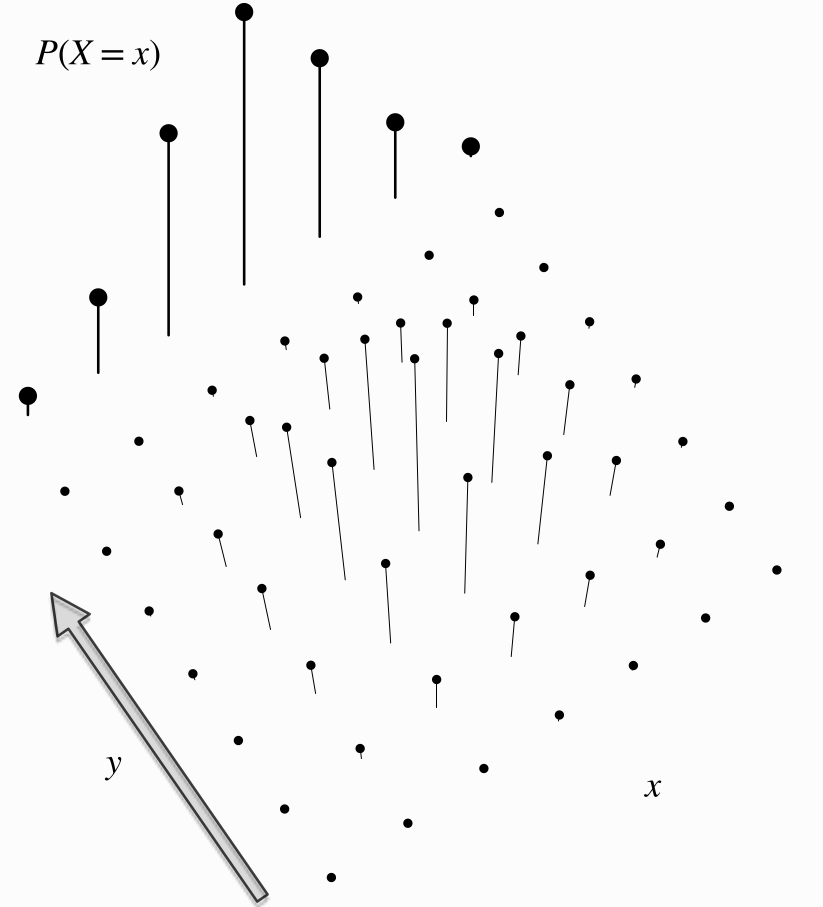
\includegraphics[scale = .25]{Images/marginal_PMF.png}
    \caption{Figure above shows the process of obtaining the marginal PMF from the joint PMF. Here we take a bird's-eye view of the joint PMF for a clearer perspective; each column of the joint PMF corresponds to a fixed $x$ and each row corresponds to a fixed $y$. For any $x$, the probability $\mathbb{P}(X=x)$ is the total height of the bars in the corresponding column of the joint PMF: we can imagine taking all the bars in that column and stacking them on top of each other to get the marginal probability. Repeating this for all $x$, we arrive at the marginal PMF, depicted in bold.}
\end{figure}

\end{frame}

\begin{frame}{Marginal Expectations and Variance}

\begin{itemize}
  \item So from joint PMF of two random variables $X$ and $Y$, we can calculate marginal PMFs, $f_{X}(x)$ and $f_{X}(y)$ and using these marginal PMFs we can calculate marginal expectations, $\mathbb{E}(X)$ and $\mathbb{E}(Y)$. And also marginal variance $\mathrm{Var}(X)$ and $\mathrm{Var}(Y)$.

  \item Let's calculate the marginal expectation and variance using the PMF of page $16$, $17$ and $18$.

  \begin{align*}
  \begin{aligned}
  \mathbb{E}(X) &=\sum_x x f_{X}(x) =(-2)(0.27)+(0)(0.12)+(2)(0.26)+(3)(0.35) =1.03\end{aligned}
  \end{align*}
  
  \item Similarly,
  

\begin{align*}
\begin{aligned}
\mathbb{E}(Y) &=\sum_y y f_{Y}(y)=(3)(0.51)+(6)(0.49) =4.47
\end{aligned}
\end{align*}


\item Calculate $\mathrm{Var}(X)$ $\mathrm{Var}(Y)$.


\end{itemize}


\end{frame}





\subsection{Conditional PMFs, Conditional Expectation and Conditional Variance}



\begin{frame}{Conditional PMF}

\begin{itemize}
  \item Now suppose that we observe the value of $X$ and want to update our distribution of $Y$ to reflect this information. Instead of using the marginal PMF $f_{Y}(y)$, which does not take into account any information about $X$, we should use a PMF that conditions on the event $X=x$, where $x$ is the value we observed for $X$. This naturally leads us to consider conditional PMFs.

\end{itemize}

\begin{varblock}{\Thm{Definition } (Conditional PMFs)}

For discrete random variables $X$ and $Y$,

\begin{itemize}
  \item The conditional PMF of of $Y$ given $X=x$ is


  \begin{align*}
    f_{\scriptscriptstyle Y | X}(y \mid x)=\frac{f(x, y)}{f_{\scriptscriptstyle X}(x)}
  \end{align*}

  \item The conditional PMF of of $X$ given $Y=y$ is


  \begin{align*}
    f_{\scriptscriptstyle X | Y}(x \mid y)=\frac{f(x, y)}{f_{\scriptscriptstyle Y}(y)}
  \end{align*}

\end{itemize}

\end{varblock}

\begin{itemize}

  \item Note that depending on conditioning values, we will have different conditional PMFs.

  \item Note that the conditional PMF of $Y$ (for fixed $x$ ) is a valid PMF. So we can define the conditional expectation of $Y$ given $X=x$, denoted by $\mathbb{E}(Y \mid X=x)$, in the same way that we defined $\mathbb{E}(Y)$ except that we replace the PMF of $Y$ with the conditional PMF of $Y$ given $X = x$. Like any PMF, the sum of  the conditional PMF of of $Y$ given $X=x$ over all possible values of $Y$ is 1.

\end{itemize}
\end{frame}



\begin{frame}{Conditional PMF}
\Thm{Example~ }
Continuing with previous example (Example 3.3), let us compute the conditional PMF of $X$ when $Y = 3$, so we need $f_{\scriptscriptstyle X | Y}(x|3)$. This means we need to calculate $f_{\scriptscriptstyle X | Y}(-2|3), f_{\scriptscriptstyle X | Y}(0|3), f_{\scriptscriptstyle X | Y}(2|3)$ and $f_{\scriptscriptstyle X | Y}(3|3)$. 

\begin{align*}
f_{\scriptscriptstyle X | Y}(-2 \mid 3)=\frac{f(-2, 3)}{f_{\scriptscriptstyle Y}(3)}=0.27 / 0.51=0.53
\end{align*}

We can also calculate 

\begin{align*}
 f_{\scriptscriptstyle X | Y}(0|3), f_{\scriptscriptstyle X | Y}(2|3) \text{ and }  f_{\scriptscriptstyle X | Y}(3|3).
\end{align*}

\begin{itemize}
  \item Now because conditional PMF is a valid PMF, we will have $ f_{\scriptscriptstyle X | Y}(-2 \mid 3) + f_{\scriptscriptstyle X | Y}(0|3) + f_{\scriptscriptstyle X | Y}(2|3) +  f_{\scriptscriptstyle X | Y}(3|3) = 1$ (Try this at your home!) 

  \item Notice that the unconditional (or marginal) probability $f_{X}(-2)$ is $0.27$, but if $Y$ has assumed the value of $3$ , the probability that $X$ takes the value of $-2$ is $0.53$.
\end{itemize}






\end{frame}

\begin{frame}{Conditional PMF}

Homework: Using Example 3.3., calculate the conditional PMF $f_{\scriptscriptstyle Y | X}(y|  2)$, this means you need $f_{\scriptscriptstyle Y | X}(3|  2)$ and $f_{\scriptscriptstyle Y | X}(6|  2)$. Then calculate conditional expectation $\mathbb{E}( Y | X = 2)$, and finally calculate conditional variance $\mathrm{Var}( Y | X = 2)$.



% \begin{align*}
% f(X=2 \mid Y=6)=\frac{f(X=2, Y=6)}{f(Y=6)}=0.10 / 0.49=0.20
% \end{align*}


\end{frame}



\begin{frame}{Conditional PMF}
\begin{figure}
  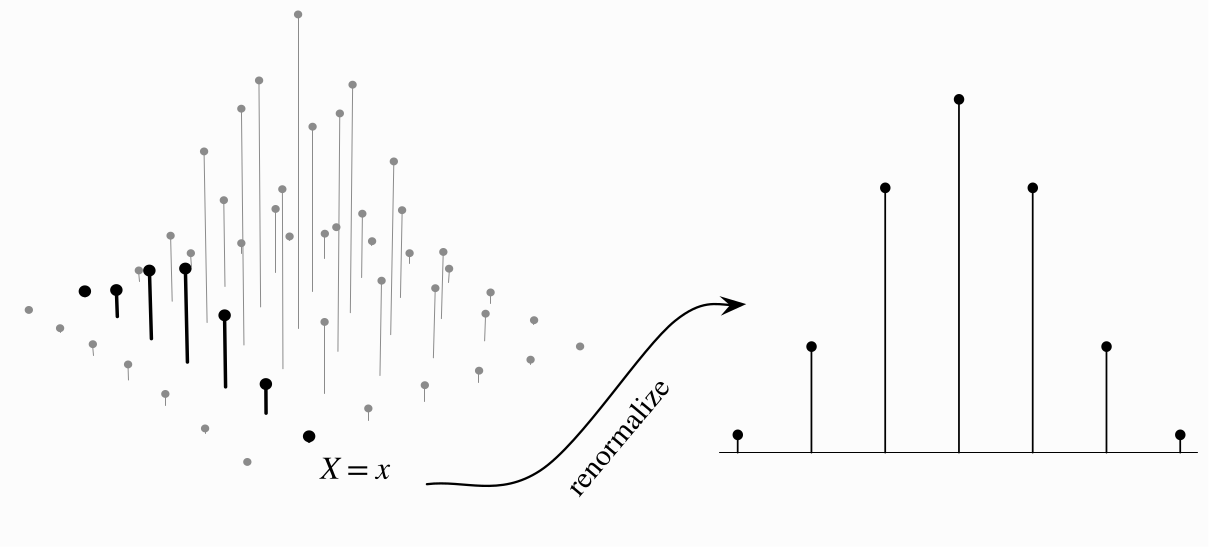
\includegraphics[scale = .25]{Images/conditional_PMF.png}
    \caption{Figure above illustrates the definition of conditional PMF. To condition on the event $X=x$, we first take the joint PMF and focus in on the vertical bars where $X$ takes on the value $x$; in the figure, these are shown in bold. All of the other vertical bars are irrelevant because they are inconsistent with the knowledge that $X=x$ occurred. Since the total height of the bold bars is the marginal probability $\mathbb{P}(X=x)$, we then renormalize the conditional PMF by dividing by $\mathbb{P}(X=x)$; this ensures that the conditional PMF will sum to 1. Therefore conditional PMFs are PMFs, just as conditional probabilities are probabilities. Notice that there is a different conditional PMF of $Y$ for every possible value of $X$; Figure above highlights just one of these conditional PMFs.}
\end{figure}

\end{frame}


\subsection{Independence of two discrete random variables}

\begin{frame}{Independence of discrete random variables}
We earlier discussed independence of events. Armed with an understanding of joint, marginal, and conditional distributions, we can revisit the definition of independence for random variables.


\begin{varblock}{\Thm{Definition } (Independence of discrete random variables)}
If $X$ and $Y$ are discrete random variables, then $X$ and $Y$ are \alert{independent} if for all $x$ and $y$,


\begin{align*}
\mathbb{P}(X=x, Y=y)=\mathbb{P}(X=x) \mathbb{P}(Y=y)
\end{align*}
for all $x$ and $y$. Note that, this means


\begin{align*}
f(x,y)=f_{X}(x) f_{Y}(y)
\end{align*}

for all $x$ and $y$

\end{varblock}

\begin{itemize}


   \item The definition says that for independent r.v.s, the joint PMF factors into the product of the marginal PMFs. 

 \end{itemize} 

\end{frame}


\begin{frame}{Independence of discrete random variables}

\begin{itemize}
   \item Remember! in general, the marginal distributions do not determine the joint distribution.

   \item This means joint distribution comes first, and this is the entire reason why we wanted to study joint distributions in the first place! 

   \item But in the case of independence, the marginal distributions are all we need to specify the joint distribution.

   \item Try to construct a joint PMF of $X$ and $Y$ after constructing Marginal PMFs of $X$ and $Y$ such that the two random variables are independnt. 

   \item Another way of looking at independence is that all the conditional PMFs are the same as the marginal PMF (why is that?), becuase if two random variables are independent conditional probabilities are same as marginal probabilities.

   \item In other words, starting with the marginal PMF of $Y$, no updating is necessary when we condition on $X=x$, regardless of what $x$ is. 
 \end{itemize} 

\end{frame}


\begin{frame}{Independence of discrete random variables}

\Thm{Example~ }
Show that, $X$ and $Y$ variables whose joint given in Example 3.3 are NOT independent (Note: Finding even one pair of values $x$ and $y$ such that $f(x,y) \neq f_{X}(x)f_{X}(y)$ is enough to rule out independence.)

% \Thm{Example~ }
% A bag contains three balls numbered 1, 2, and 3. Two balls are drawn at random, with replacement, from the bag (i.e., the first ball drawn is replaced before the second is drawn). Let $X$ denote the number of the first ball drawn and $Y$ the number of the second ball drawn. The following table gives the joint PDF of $X$ and $Y$.

% \begin{table}
% \centering
% \begin{tabular}{ccccc}
% \hline & & \multicolumn{3}{c}{$X$} \\
% \cline { 3 - 5 } & ${1}$ & ${2}$ & ${3}$ \\
% \hline & ${1}$ & $\frac{1}{9}$ & $\frac{1}{9}$ & $\frac{1}{9}$ \\
% $Y$ & ${2}$ & $\frac{1}{9}$ & $\frac{1}{9}$ & $\frac{1}{9}$ \\
% & ${3}$ & $\frac{1}{9}$ & $\frac{1}{9}$ & $\frac{1}{9}$ \\
% \hline
% \end{tabular}  
% \end{table}



% Now $f(X=1, Y=1)=\frac{1}{9}, f(X=1)=\frac{1}{3}$ (obtained by summing the first column), and $f(Y=1)=\frac{1}{3}$ (obtained by summing the first row). Since $f(X, Y)=f_{X}(X) f_{X}(Y)$ in this example we can say that the two variables are statistically independent. It can be easily checked that for any other combination of $X$ and $Y$ values given in the above table the joint PDF factors into individual PDFs.

\end{frame}


\subsection{Idea of Covariance for two ranadom variables}

\begin{frame}{Covariance and Correlation}
\begin{varblock}{\Thm{Definition~ } (Covariance and Correlation) }

The covariance between two random variables $X$ and $Y$ is
\begin{align*}
\operatorname{Cov}(X, Y)=\mathbb{E}\left[\left(X-\mathbb{E}(X)\right)\left(Y-\mathbb{E}(Y)\right)\right] = \mathbb{E}\left[\left(X- \mu_{X}\right)\left(Y-\mu_Y\right)\right]
\end{align*}

And the Correlation between two random variables $X$ and $Y$ is

\begin{align*}
  \operatorname{Cor}(X, Y) = \frac{\operatorname{Cov}(X, Y)}{ \left(\sqrt{\mathrm{Var}(X)}\right) \left(\sqrt{\mathrm{Var}(Y)}\right) } = \frac{\operatorname{Cov}(X, Y)}{ \sigma_X \times \sigma_Y }
\end{align*}


\end{varblock}

\begin{itemize}

  \item where $\mu_X$ and $\mu_Y$ are the marginal Expected values of $X$ and $Y$, and  $\sigma_X$ and $\sigma_Y$ are the standard deviations of $X$ and $Y$.

  \item Notice if the covariance is $0$, then correlation is also $0$.

  \item Sometimes $\rho_{X, Y}$ is used for correlation.

  \item Notice $ -1 \leq \operatorname{Cor}(X, Y) \leq 1$, this is the benefit of correlation that it gives a value between $-1$ and $1$, but what does this mean.

  \item Let's understand Covariance first, then we will understand Correlation.


 
  \end{itemize}

\end{frame}




\begin{frame}{Covariance and Correlation}


\begin{itemize}



  \item Let's think about the definition intuitively. If $X$ and $Y$ tend to move in the same direction, then $X- \mathbb{E}(X)$ and $Y-\mathbb{E}(Y)$ will tend to be either both positive or both negative, so $(X-\mathbb{E}(X))(Y-\mathbb{E}(Y))$ will be positive on average, giving a positive covariance. 


  \item If $X$ and $Y$ tend to move in opposite directions, then $X-\mathbb{E}(X)$ and $Y-\mathbb{E}(Y)$ will tend to have opposite signs, giving a negative covariance.

  \item If $X$ and $Y$ are independent, we can show that their covariance is zero (we will see why later!). 

  \item We say that random variables with zero covariance are \alert{uncorrelated}. We will come back to this again after we see an example.


    \item For the covariance , we have an equivalent expression:
    \begin{align*}
    \operatorname{Cov}(X, Y)=\mathbb{E}(X Y)-\mathbb{E}(X) \mathbb{E}(Y)
    \end{align*}

  \end{itemize}

\end{frame}

\begin{frame}{Covariance and Correlation}
\Thm{Example~ } 

Let us find out the covariance between discrete random variables $X$ and $Y$ whose joint PMF is as shown in Example 3.3. This is a tedious calculation, but you should use the following formula,

\begin{align*}
  \operatorname{Cov}(X, Y)&=\mathbb{E}\left[\left(X-\mathbb{E}(X)\right)\left(Y-\mathbb{E}(Y)\right)\right] \\
  &= \sum_{x}\sum_{y} \left[\left(x - \mathbb{E}\left(X\right)\right) \left(y - \mathbb{E}\left(Y\right)\right)\right] \times f(x, y)
\end{align*}

It should be $2.24$



% From Example 3.10 we already know that $\mathbb{E}(X)=1.03$ and $\mathbb{E}(Y)=4.47$. From Example 3.12 we know that $\mathbb{E}(XY)=6.84$. Therefore,
%   \begin{align*}
%   \begin{aligned}
%   \operatorname{Cov}(X, Y) &=\mathbb{E}(X Y)-\mathbb{E}(X)\mathbb{E}(Y) \\
%   &=6.84-(1.03)(4.47) \\
%   &=2.24
%   \end{aligned}
%   \end{align*}
\end{frame}



\begin{frame}{Expectation of function of $X$ and $Y$}

The two-dimensional version of LOTUS lets us calculate the expectation of a random variable that is a function of two random variables $X$ and $Y$, using the joint distribution of $X$ and $Y$.

\begin{varblock}{\Thm{Theorem~ } (2D LOTUS Discrete) }

Let $g$ be a function from $\mathbb{R}^2$ to $\mathbb{R}$. If $X$ and $Y$ are discrete, then

\begin{align*}
  \mathbb{E}(g(X, Y))=\underset{{ }}{\sum \sum} g(x, y) f(x,y)
\end{align*}

\end{varblock}
\end{frame}


\begin{frame}{Expectation of function of $X$ and $Y$}

\Thm{Example~ } 
Let us find $\mathbb{E}(X,Y)$ from the joint PMF given in Example 3.3. 

$$\begin{aligned}
\mathbb{E}(XY)=& \underset{{ }}{\sum_x \sum_y} xy f(x, y) \\
=&(-2)(3)(0.27)+(0)(3)(0.08)+(2)(3)(0.16)+(3)(3)(0) \\
&+(-2)(6)(0)+(0)(6)(0.04)+(2)(6)(0.10)+(3)(6)(0.35) \\
=& 6.84
\end{aligned}$$

We can also verify previous calculation

  \begin{align*}
  \begin{aligned}
  \operatorname{Cov}(X, Y) &=\mathbb{E}(X Y)-\mathbb{E}(X)\mathbb{E}(Y) \\
  &=6.84-(1.03)(4.47) \\
  &=2.24
  \end{aligned}
  \end{align*}

\end{frame}



% \begin{frame}{Linearity of Expectaton of Discrete Random Variables}
% \begin{itemize}
%   \item Let $X$ and $Y$ be discrete random variables.  By 2D LOTUS,
% \begin{align*}
% \begin{aligned}
% \mathbb{E}(X+Y) &=\underset{{ }}{\sum \sum}(x+y) f(x, y)  \\
% &=\underset{{ }}{\sum \sum} x f(x, y)+\underset{{ }}{\sum \sum}y f(x, y)  \\
% &=\sum_x  x\sum_y f(x, y)+\sum_y  y\sum_x f(x, y)  \\
% &=\sum_x  xf_{X}(x)+\sum_y  yf_{X}(y) \quad \text{[Marginalize]} \\
% &=\mathbb{E}(X)+\mathbb{E}(Y)
% \end{aligned}
% \end{align*}


% \item Note: More generally $X_1, X_2, \ldots, X_N$ are $N$ random variables and $a_1, a_2, \ldots, a_N$ and $b$ are constants, then
% \begin{align*}
% \mathbb{E}\left(a_1 X_1+a_2 X_2+\cdots+a_N X_N+b\right)=a_1 \mathbb{E}\left(X_1\right)+a_2 \mathbb{E}\left(X_2\right)+\cdots+a_N \mathbb{E}\left(X_N\right)+b
% \end{align*}
% \end{itemize}




% \end{frame}





\begin{frame}{Covariance and Independence}
\begin{varblock}{\Thm{Theorem~ }  }
If $X$ and $Y$ are independent, then they are uncorrelated.

\end{varblock}

\begin{itemize}
  \item This can be easily show for two discrete random variables $X$ and $Y$. If $X$ and $Y$ are independent, their joint PDF is the product of the marginal PDFs $f(x,y) = f_{X}(x)f_{X}(y)$. By 2D LOTUS,

  \begin{align*}
  \begin{aligned}
  \mathbb{E}(X Y) &=\underset{{ }}{\sum_x \sum_y}  x y f_{X}(x) f_{X}(y)  =\sum_x x f_X(x)  \sum_y y f_{X}(y) =\mathbb{E}(X) \mathbb{E}(Y) .
  \end{aligned}
  \end{align*}
which gives 
\begin{align*}
\operatorname{Cov}(X, Y)=\mathbb{E}(X Y)-\mathbb{E}(X) \mathbb{E}(Y)=0-0=0
\end{align*}

\item CAREFUL! The converse of this theorem is false: just because $X$ and $Y$ are uncorrelated does not mean they are independent.


\item Covariance is a measure of linear association, so r.v.s can be dependent in nonlinear ways and still have zero covariance. We see an example of that below


\end{itemize}
\end{frame}

\begin{frame}{Covariance and Independence}

\Thm{Example~ }
Suppose that the random variable $X$ has probability distribution
\begin{align*}
\mathbb{P}(-1)=1 / 4 \quad \mathbb{P}(0)=1 / 2 \quad \mathbb{P}(1)=1 / 4
\end{align*}
Let the random variable $Y$ be defined as follows:
\begin{align*}
Y=X^2
\end{align*}
Thus, knowledge of the value taken by $X$ implies knowledge of the value taken by $Y$, and, therefore, these two random variables are certainly not independent. Whenever $X=0$, then $Y=0$, and if $X$ is either $-1$ or 1 , then $Y=1$. The joint probability distribution of $X$ and $Y$ is
\begin{align*}
\mathbb{P}(-1,1)=1 / 4 \quad \mathbb{P}(0,0)=1 / 2 \quad \mathbb{P}(1,1)=1 / 4
\end{align*}
with the probability of any other combination of values being equal to 0 . It is then straightforward to verify that
\begin{align*}
E[X]=0 \quad E[Y]=1 / 2 \quad E[X Y]=0
\end{align*}
The covariance between $X$ and $Y$ is 0 . Thus we see that random variables that are not independent can have a covariance equal to 0 .

\end{frame}





% \subsection{Moments}





\begin{frame}[allowframebreaks]{References}
\vspace*{.3cm} 

\scriptsize
% \printbibliography[maxnames=99]

% \nocite{*}
\bibliographystyle{apalike}
\bibliography{../common/references}  
% \nocite{*}

\end{frame}

\end{document}
